\documentclass[aspectratio=149,11pt]{beamer}
\usetheme{CERNship}
\graphicspath{{figs/}}
% Style: plot-centred, <= 3 short bullets per figure, one grey \slidenote.
% Source: Background Tagging report (Gfrisella/Background_Tagging_Report, 16 Nov 2026) and the reco runs in
% Optimization_Veto_System/veto/results_rerun/reco (R1/R2/R3, full Nov-4 sample). The fin designs are examples only.

\newcommand{\pend}[1]{\textcolor{red}{#1}}

\title{Background Tagger for the SHiP decay volume}
\subtitle{Background without tagging, reference designs R1 / R2 / R3, and the road to the optimisation}
\shorttitle{SHiP BT status}
\author{\underline{Guglielmo Frisella}\,\textsuperscript{1, 2}}
\institute{\textsuperscript{1}University of Zurich\\[2pt]
           \textsuperscript{2}European Organization for Nuclear Research (CERN)}
\date{November 17, 2026}

\begin{document}

\cernCover

\begin{frame}
  \titlepage
\end{frame}

\begin{frame}{Outline}
  \tableofcontents
\end{frame}

% ============================================================
\section{Sample and selection}
% ============================================================
\begin{frame}{Sample, normalisation and selection}
  \begin{columns}[T]
    \begin{column}{0.55\textwidth}
      \small
      \begin{itemize}\setlength{\itemsep}{2pt}
        \item Full Nov-4 muon production: 3\,220 spills
        \item \SI{4e13}{PoT} per spill; 15\,y $=$ \num{1.5e7} spills
        \item FairShip layout 2026-0.1, shield TRY6
        \item $\geq 2$ good tracks at SST1, $p > \SI{1}{GeV}$, timing acceptance
        \item Full selection (F): IP $< \SI{10}{cm}$
        \item Partial selection (P): IP $< \SI{2.5}{m}$
      \end{itemize}
    \end{column}
    \begin{column}{0.41\textwidth}
      \footnotesize
      \begin{tabular}{@{}l@{\hspace{4pt}}r@{}}
        \toprule
        Shield end (MS7)  & \SI{29.89}{m} \\
        UBT straws        & \SI{30.73}{m} \\
        UBT tiles, window & \SI{31.13}{m} \\
        Vessel            & 31.13--\SI{81.13}{m} \\
        SST1              & \SI{82.08}{m} \\
        \midrule
        Candidate $\mu\mu$ pairs & \num{215500} \\
        \quad pass F / P   & \num{42390} / \num{215188} \\
        \bottomrule
      \end{tabular}
    \end{column}
  \end{columns}
  \slidenote{Yield per 15 y $= N_\mathrm{spill}\sum_{i\in\mathrm{sel}} w_i$, error $N_\mathrm{spill}(\sum w_i^2)^{1/2}$, parents resampled when events share a muon.}
\end{frame}

\begin{frame}{Muon flux at the vessel entrance}
  \centering
  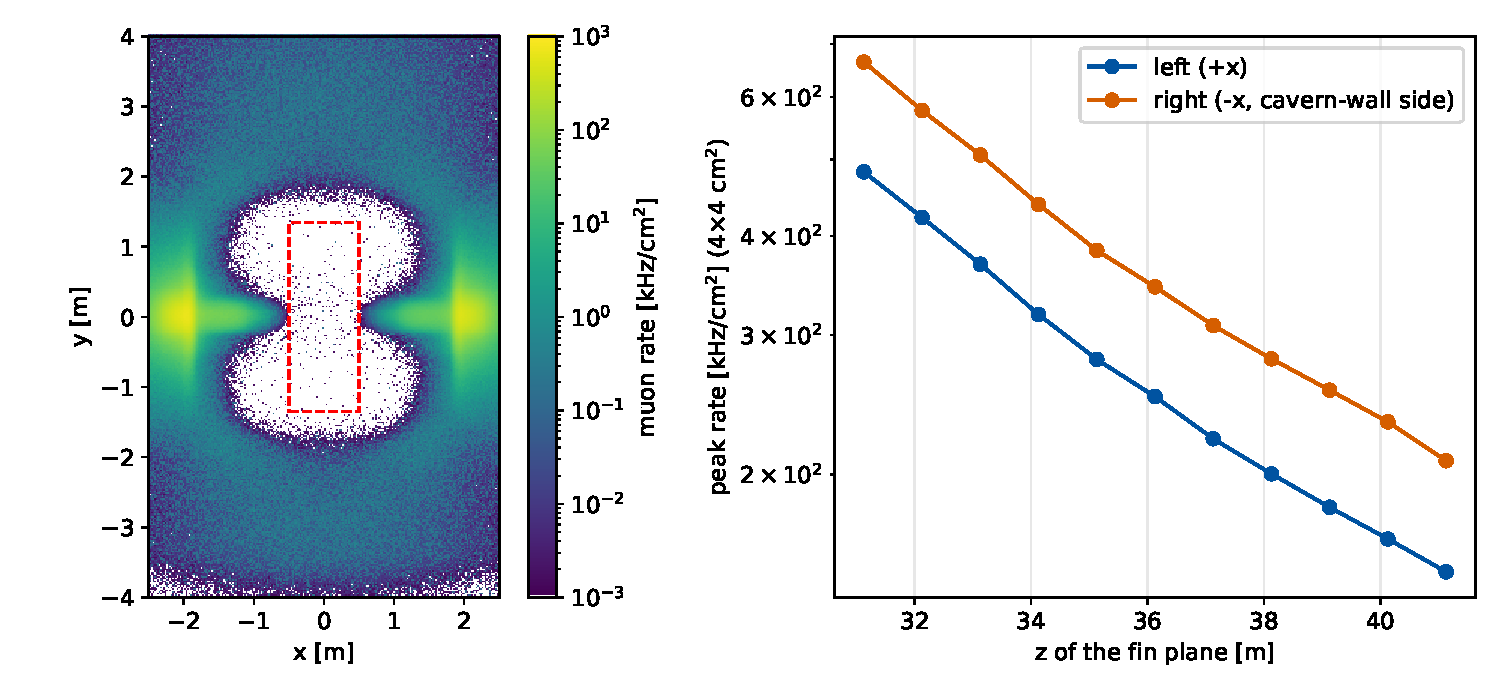
\includegraphics[width=0.92\textwidth]{report/bt_entrance_rates.pdf}
  \begin{itemize}\footnotesize
    \item $1.3\times10^{9}$ muons per spill on the tile plane, almost all in the flames ($|y| \lesssim \SI{0.5}{m}$)
    \item Peak \SI{0.66}{MHz/cm^2} on the cavern-wall side; only \num{1e4} per spill through the window
  \end{itemize}
  \slidenote{Left: rate at $z = \SI{31.13}{m}$; dashed red: entrance window. Right: peak rate on fins at 31--\SI{41}{m}.}
\end{frame}

% ============================================================
\section{Background without tagging}
% ============================================================
\begin{frame}{Background per 15 years, before tagging}
  \centering
  \footnotesize
  \begin{tabular}{@{}lcc@{}}
    \toprule
    Source & full (IP $< \SI{10}{cm}$) & partial (IP $< \SI{2.5}{m}$) \\
    \midrule
    Combinatorial $\mu \times \mu$                 & $2.36 \pm 0.52$ & $34.4 \pm 2.1$ \\
    Combinatorial (MS7 V0 product) $\times \mu$     & 62.7 & -- \\
    Combinatorial (cavern-rock track) $\times \mu$  & 211 & \pend{pending} \\
    Muon inelastic: vessel, walls, tagger, air      & $2370 \pm 110$ & $(2.21 \pm 0.04)\times10^{4}$ \\
    Muon inelastic: MS7 ($K_L$)                     & \pend{$(6.1 \pm 4.3)\times10^{4}$} & \pend{$1.39\times10^{7}$} \\
    Neutrino inelastic: vessel, walls, tagger, air  & $7.0 \pm 0.5$ & $660 \pm 5$ \\
    Neutrino inelastic: MS7                         & $9.9 \pm 6.8$ & $1390 \pm 170$ \\
    \bottomrule
  \end{tabular}
  \slidenote{After the selection, no tagger information. Red: MS7 muon V0 rests on two simulated events; a V0-enriched generation is replacing it (D16). Cavern rock $\times$ rock not evaluated.}
\end{frame}

\begin{frame}{Inelastic scattering by target (full selection)}
  \begin{columns}[T]
    \begin{column}{0.49\textwidth}
      \footnotesize
      Muons, IP $< \SI{10}{cm}$ / 15\,y\\[2pt]
      \begin{tabular}{@{}lr@{}}
        \toprule
        Helium               & $1753 \pm 47$ \\
        Vessel walls         & $265 \pm 77$ \\
        Tagger material (UBT) & $350 \pm 67$ \\
        Air, around / upstream & 0 / $1.8$ \\
        MS7 iron, $K_L$       & \pend{$(6.1 \pm 4.3)\times10^{4}$} \\
        \bottomrule
      \end{tabular}
    \end{column}
    \begin{column}{0.47\textwidth}
      \footnotesize
      Neutrinos, IP $< \SI{10}{cm}$ / 15\,y\\[2pt]
      \begin{tabular}{@{}lr@{}}
        \toprule
        Helium               & $3.61 \pm 0.19$ \\
        Vessel walls         & $0.021$ \\
        Tagger material (UBT) & $3.37 \pm 0.51$ \\
        Air                  & $0.03$ \\
        MS7 iron             & $9.9 \pm 6.8$ \\
        \bottomrule
      \end{tabular}
    \end{column}
  \end{columns}
  \vspace{0.3cm}
  \begin{itemize}\small
    \item Muon interactions in the vessel: the parent crosses the tagger, taggable
    \item MS7 $K_L$ and $\nu$ in the helium: no charged parent, irreducible for a tagger
  \end{itemize}
  \slidenote{2026 neutrino flux, all six flavours. The UBT tile plane on the window is a target as large as the helium for neutrinos.}
\end{frame}

\begin{frame}{$K_L$ from the shield: generators}
  \centering
  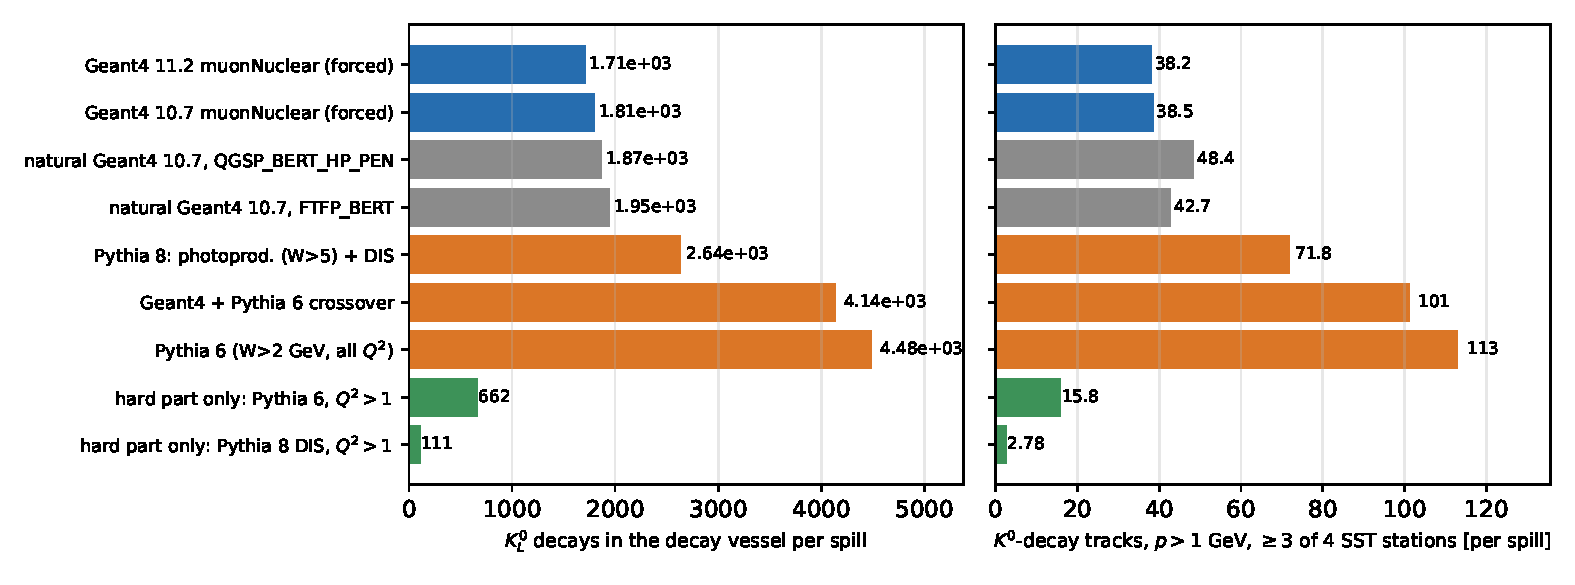
\includegraphics[width=0.92\textwidth]{report/int_generators_kl.pdf}
  \begin{itemize}\footnotesize
    \item Geant4 muonNuclear (default) agrees with natural Geant4 and with $\gamma p$ data ($\sim$6\,\%)
    \item Pythia-based chains $\times 1.5$--2.5 higher: generator spread one-sided, $+20\,\%$
  \end{itemize}
  \slidenote{Per spill. Left: $K^0$ decays in the decay vessel; right: $K^0$-decay tracks with $p > \SI{1}{GeV}$ in $\geq 3$ of 4 SST1 stations.}
\end{frame}

% ============================================================
\section{Reference designs R1 / R2 / R3}
% ============================================================
\begin{frame}{The reference designs}
  \begin{columns}[T]
    \begin{column}{0.55\textwidth}
      \small
      \begin{itemize}\setlength{\itemsep}{3pt}
        \item \textbf{R1}: UBT only (vertical straws + $4\times4$\,m$^2$ tiles)
        \item \textbf{R2}: R1 $+$ full SBT (854 cells, 4 walls)
        \item \textbf{R3}: R2 $+$ V0 rule $+$ 3 layers of Si strips in MS7
        \item Costs in drachmas: 1 = one $0.5\times0.5$\,m$^2$ tile module
        \item Budget $=$ cost of R2
      \end{itemize}
    \end{column}
    \begin{column}{0.41\textwidth}
      \footnotesize
      \begin{tabular}{@{}lrr@{}}
        \toprule
        Design & channels & drachmas \\
        \midrule
        R1 & \num{18100}  & 99.7 \\
        R2 & \num{31764}  & 333.5 \\
        R3 & \num{108564} & 378.7 \\
        \bottomrule
      \end{tabular}\\[4pt]
      R3: $+13.6\,\%$ over the budget
    \end{column}
  \end{columns}
  \slidenote{Tiles: $2\times2$\,cm$^2$ in the flame blocks ($1 \leq |x| \leq \SI{2}{m}$, $|y| \leq \SI{0.6}{m}$), $4\times4$\,cm$^2$ elsewhere; tagging window $\pm3\sigma$. SBT: \SI{20}{cm} liquid scintillator, \SI{30}{MeV} threshold, pointing association.}
\end{frame}

\begin{frame}{Evaluation on the full sample}
  \centering
  \footnotesize
  \begin{tabular}{@{}lcccccc@{}}
    \toprule
    Design & \multicolumn{2}{c}{$\mu\mu$ pairs / 15\,y} & \multicolumn{2}{c}{signal lost} & selected $\mu$ & all SST1 $\mu$ \\
           & F & P & F & P & tagged & tagged \\
    \midrule
    R1 & $< \num{1.3e-4}$ & \num{2.7e-8} & 3.1\,\% & 3.0\,\% & 97.7\,\% & 65.8\,\% \\
    R2 & $< \num{1.3e-4}$ & $< \num{3.7e-4}$ & 3.2\,\% & 2.9\,\% & 100.0\,\% & 92.1\,\% \\
    R3 & $< \num{1.3e-4}$ & $< \num{3.7e-4}$ & \pend{24.6\,\%} & \pend{25.8\,\%} & 100.0\,\% & 93.7\,\% \\
    \bottomrule
  \end{tabular}\\[6pt]
  \begin{itemize}\small
    \item $\mu\mu$ pairs (2.36 / 34.4 before) removed already by R1 with the $\pm3\sigma$ tile window
    \item Signal loss of R1/R2 mostly from the UBT straws (EM debris in their \SI{25}{ns} window)
  \end{itemize}
  \slidenote{\texttt{run\_reco}, full Nov-4 sample, EventCalc signal benchmarks, EM debris on. ``$<$'': no surviving pair, 1$\sigma$ weight bound. Red: the R3 signal loss (V0 rule) is under study; MS7 V0 columns follow the V0-enriched sample.}
\end{frame}

% ============================================================
\section{Example: fins instead of the SBT}
% ============================================================
\begin{frame}{Example designs: R2-fins and R3-fins (not references)}
  \centering
  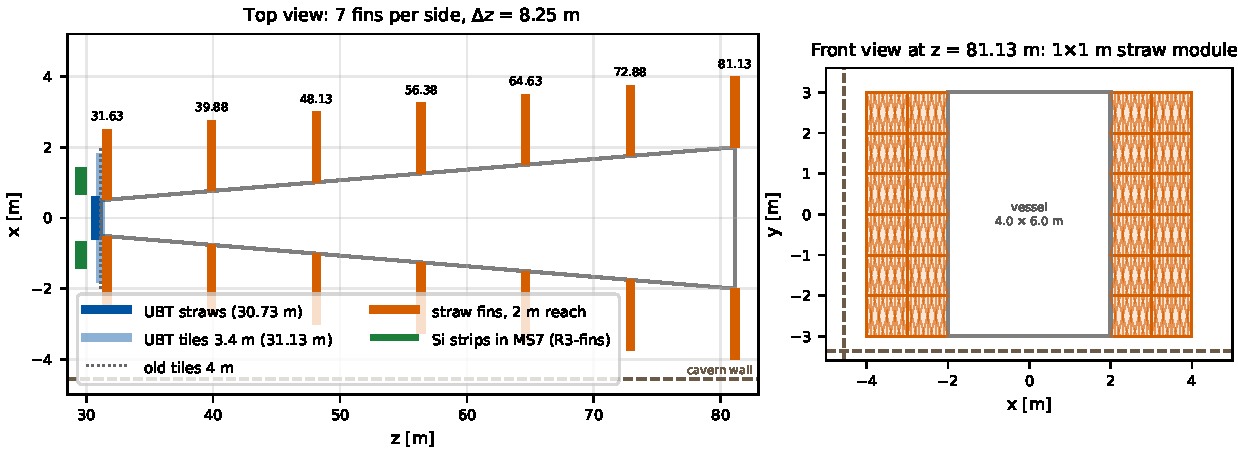
\includegraphics[width=0.96\textwidth]{fins/fin_layout.pdf}
  \begin{itemize}\footnotesize
    \item R2 / R3 without the SBT; 7 straw fins per side from \SI{81.13}{m} to \SI{31.63}{m}, 2 m reach, vessel height
    \item UBT tile plane reduced from $4\times4$ to $3.4\times2.7$\,m$^2$
  \end{itemize}
  \slidenote{Straw modules $1\times1$\,m$^2$, three stereo views (0, $\pm15^\circ$), on the 50\,cm grid. Only examples of what a tagger with fins gives; the optimisation starts from R1 / R2 / R3.}
\end{frame}

\begin{frame}{Example designs: results}
  \centering
  \footnotesize
  \begin{tabular}{@{}lccccrr@{}}
    \toprule
    Design & \multicolumn{2}{c}{$\mu\mu$ pairs / 15\,y} & \multicolumn{2}{c}{signal lost} & channels & drachmas \\
           & F & P & F & P & & \\
    \midrule
    R1 & $< \num{1.3e-4}$ & \num{2.7e-8} & 3.1\,\% & 3.0\,\% & \num{18100} & 99.7 \\
    R2 & $< \num{1.3e-4}$ & $< \num{3.7e-4}$ & 3.2\,\% & 2.9\,\% & \num{31764} & 333.5 \\
    \midrule
    R2-fins & $< \num{1.3e-4}$ & $0.0017 \pm 0.002$ & \textbf{16.7\,\%} & \textbf{18.0\,\%} & \num{193368} & 439.7 \\
    R3-fins & $< \num{1.3e-4}$ & $< \num{3.7e-4}$ & \textbf{71.9\,\%} & \textbf{69.6\,\%} & \num{270168} & 484.9 \\
    \bottomrule
  \end{tabular}\\[6pt]
  \begin{itemize}\small
    \item Fin at \SI{31.63}{m} sits in the flames: 12--\SI{16}{MHz} per straw, over the \SI{0.5}{MHz} limit
    \item It causes most of the signal loss; with the V0 rule every fin hit can tag a signal vertex
  \end{itemize}
  \slidenote{Same evaluation as R1 / R2 (full Nov-4 sample, EventCalc signal, EM debris; tile EM map cropped to $3.4\times2.7$\,m$^2$). All SST1 muons tagged: 93.8\,\% (R2-fins), 92.1\,\% (R2). A layout to be optimised, not a candidate.}
\end{frame}

% ============================================================
\section{Next steps}
% ============================================================
\begin{frame}{Next step: optimisation with AlphaEvolve}
  \begin{columns}[T]
    \begin{column}{0.52\textwidth}
      \small
      \begin{itemize}\setlength{\itemsep}{3pt}
        \item AlphaEvolve proposes layouts; each is scored by the full chain
        \item Score: background after tagging, signal loss, cost vs budget
        \item Rate limits per technology as penalties
        \item Start from R1 / R2 / R3; fin layouts are part of the search space
      \end{itemize}
    \end{column}
    \begin{column}{0.44\textwidth}
      \footnotesize
      \begin{tabular}{@{}ll@{}}
        \toprule
        Parameter & range \\
        \midrule
        Entrance plane & $y$ extent, stations \\
        Fins & side, $z$, reach, $y$ range \\
        Technology & per 50\,cm slot \\
        Bottom panel & optional \\
        Bounce search & scanned range \\
        \bottomrule
      \end{tabular}
    \end{column}
  \end{columns}
  \slidenote{Inputs: \texttt{inputs\_nov4full} pairs and the prepared interaction caches (\texttt{\_nov4full}); a 5 generations $\times$ 8 children trial first.}
\end{frame}

\begin{frame}{Summary}
  \begin{itemize}
    \item Before tagging: MS7 $K_L$ dominates, \textbf{\pend{$\sim$\num{6e4}} / 15 y} (full selection, pending)
    \item Vessel muon interactions \textbf{2370 / 15 y}: taggable, the parent crosses the tagger
    \item $\mu\mu$ pairs removed by all reference designs; signal loss \textbf{3\,\%} for R1 / R2
    \item Fins instead of the SBT (example): tag as well as R2, but a fin in the flames costs \textbf{17\,\%} of the signal
  \end{itemize}
  \vspace{0.3cm}
  \textbf{Next steps}
  \begin{itemize}
    \item V0-enriched MS7 sample $\to$ MS7 rows and R1 / R2 / R3 MS7 columns
    \item SBT as a target (D19) and R3 signal loss
    \item AlphaEvolve optimisation from R1 / R2 / R3
  \end{itemize}
\end{frame}

\end{document}
